% !TeX root = ../thuthesis-example.tex

\chapter{编译算法优化}
\thusetup{
  cite-style = super,
}

\section{灵活规约语义提升}\label{sec:compiler-alg-intro}
首先,~\ref{sec:reduction-core}节证明了规约是稀疏稠密混合代数的核心操作。稀疏稠密混合代数包括诸如SpMM,SDDMM,MTTKRP,TTM等多种算子。从这一核心观察出发,基于~\ref{sec:hwmodel}节描述的硬件模型,和~\ref{sec:atomicparallel}节提出的原子并行来定义并行模式。
之后基于硬件模型和原子并行提出了灵活规约优化空间扩展,并以SpMM为例展示了空间扩展的构建方式。之后对灵活规约的实际性能提升做了详细的实验验证。~\ref{sec:overori}节证明了优化空间中的$\{<\frac{1}{g}\,row , c\,col>,r\}$区域和$\{<g\,nnz , c\,col>,r\}$区域经过灵活
规约扩展后可以提升原有算子的性能,~\ref{sec:overcu}节证明了灵活规约扩展后的优化空间包含性能超过官方算子库的算子。但是,~\ref{sec:exp}节的算子是人工手写的,如果向不同稀疏稠密混合代数应用灵活规约技术,需要大量工程成本,但是之前又已经通过分析
论证了灵活规约可以加速这些稀疏稠密混合代数算子。为了能以较低的成本获得灵活规约带来的性能收益,本文提出了基于灵活规约语义提升技术。这是一种基于灵活规约的编译算法,可以对任何稀疏稠密混合代数快速构建优化空间,并提供方便的性能调优接口。

当前有CUDA后端代码生成的稀疏张量编译器将线程组的语义规定为:在分块中线程的一个层级即分块语义,一个特定的并行计算单元即同步语义,或者只是一个硬件指令即硬件性质语义。例如,TACO假设将一个循环变量拆分后得到的外循环变量
设置为线程组,内循环变量设置为线程,此时线程组的大小就是分块的参数。在这里,线程组被规定为分快中线程的一个层级,没有同步语义。同时,TACO将32线程大小的线程组作为一个执行原子加法的
并行计算单元,同时假设用户在使用这一原子加法并行单元时会将最后一层循环以32为粒度拆分。在这里,线程组的执行行为是以1为步长,循环次数为32次的for循环规约。在TACO后端,一段CUDA的线程组元语比如
\textit{\_\_shfl\_down\_sync}会被发射作为上层线程组规约语义的底层实现。图~\ref{fig:sem}中以具体代码形式展示了在调度语言和底层代码两个层面的分块语义和同步语义。
\begin{figure}[h]%
  \centering
  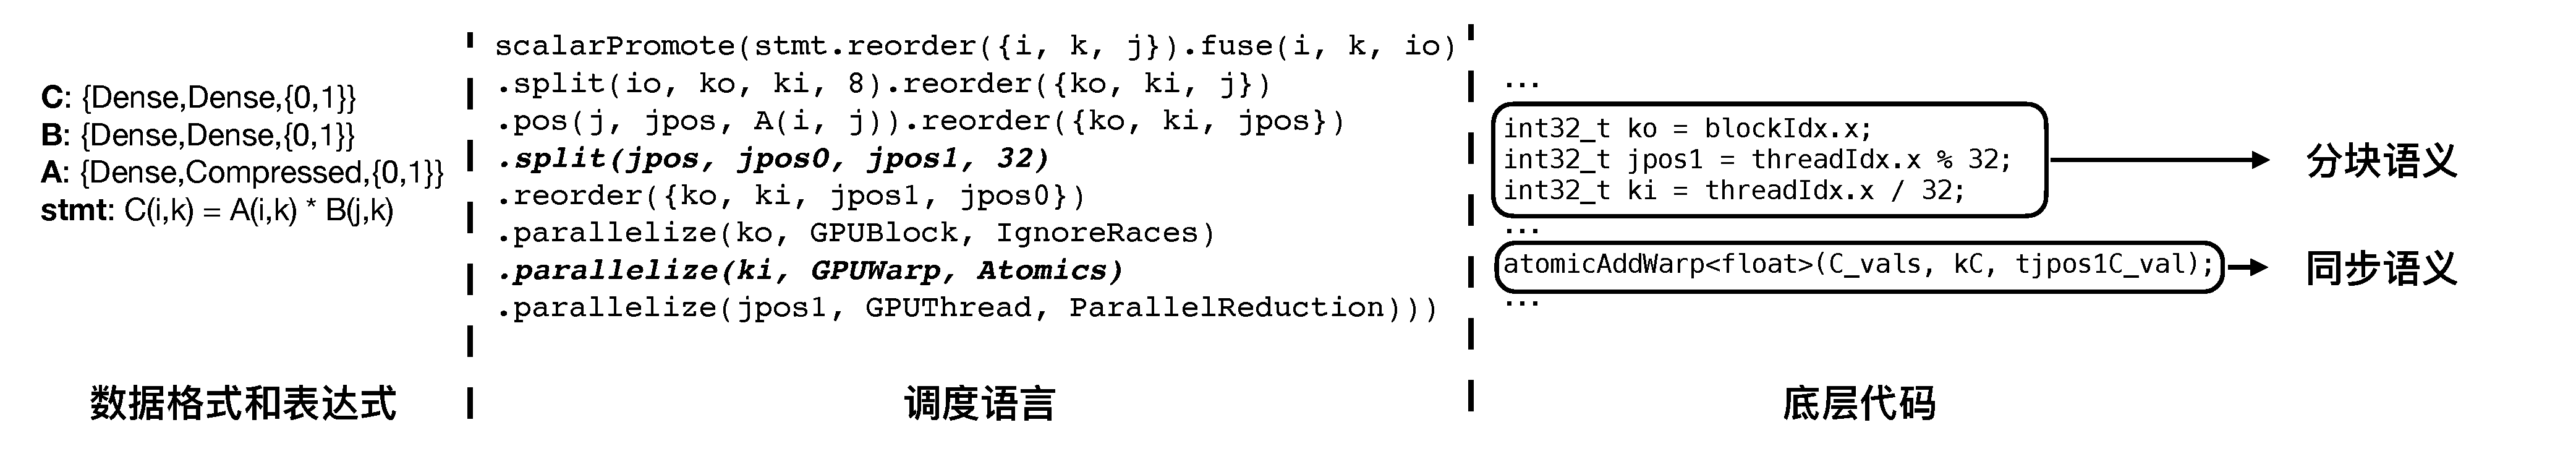
\includegraphics[width=0.99\textwidth]{semantics-cn.pdf}
  \caption{TACO中GPU线程组的分块语义和同步语义}
  \label{fig:sem}
\end{figure}
和TACO不同,TVM只将并行单元绑定在线程和线程块层级,而不会在线程组层面添加含有同步语义的调度指令。它将线程组的大小为32作为一个硬件性质,并用这一性质设置自动调度器中的调度指令参数。同时,它也将线程组作为
一个同步向共享内存或者寄存区中取数据的并行计算单元。

但是,本文提出当前稀疏算子编译器中至少有两个假设可以被突破:线程组分块和同步语义分离。以及同步语义需要可以表达灵活规约。首先,分块语义和同步语义可以被分离,因为分块语义规定了计算顺序,以及根据循环变量恢复原有角标变量
的规则,而同步语义规定的是并行模式,而并行模式规定的是计算顺序如何具体实现。因此二者是两个层面的问题,可以被分离。分块语义和同步语义需要被分离是因为在表~\ref{tab:over-sta-rb}中我们发现,SpMM在RTX 2080上
针对不同稠密矩阵列数,(4, 256, 8, 1/2)都是最佳配置,而这里分块粒度是4,同步粒度是8,二者并不相同。扩展线程组同步语义使其能表达灵活规约后,可以以很低的编程难度提升一类算子的性能。因为添加灵活规约调度指令后,就可以在调度语言层面用同一个调度指令加速加速稀疏稠密混合代数这一类算子。
再比如,SpMM优化空间中$\{<1\,nnz , x\,col>,r\}$需要同步r个线程,每个线程都在寄存器中保存了各自的行标号。因此,线程组规约应该根据行标号的不同,有不同的输出,也就是~\ref{sec:flexible-reduciton}节中的写回线程概念。
在当前稀疏算子编译器中假设只有一个写回线程,但在灵活规约扩展优化空间中写回线程可以有多个。
线程组分快和同步语义分离,和同步语义灵活规约表达不仅需要增加新的底层代码中线程组规约模板函数,也需要将灵活规约计算模式从底层代码传递到顶层调度语言中。这需要新的基本块组织方式,新的控制流和新的用户API。这些技术统称为
灵活规约语义提升技术。
\begin{figure}[h]%
  \centering
  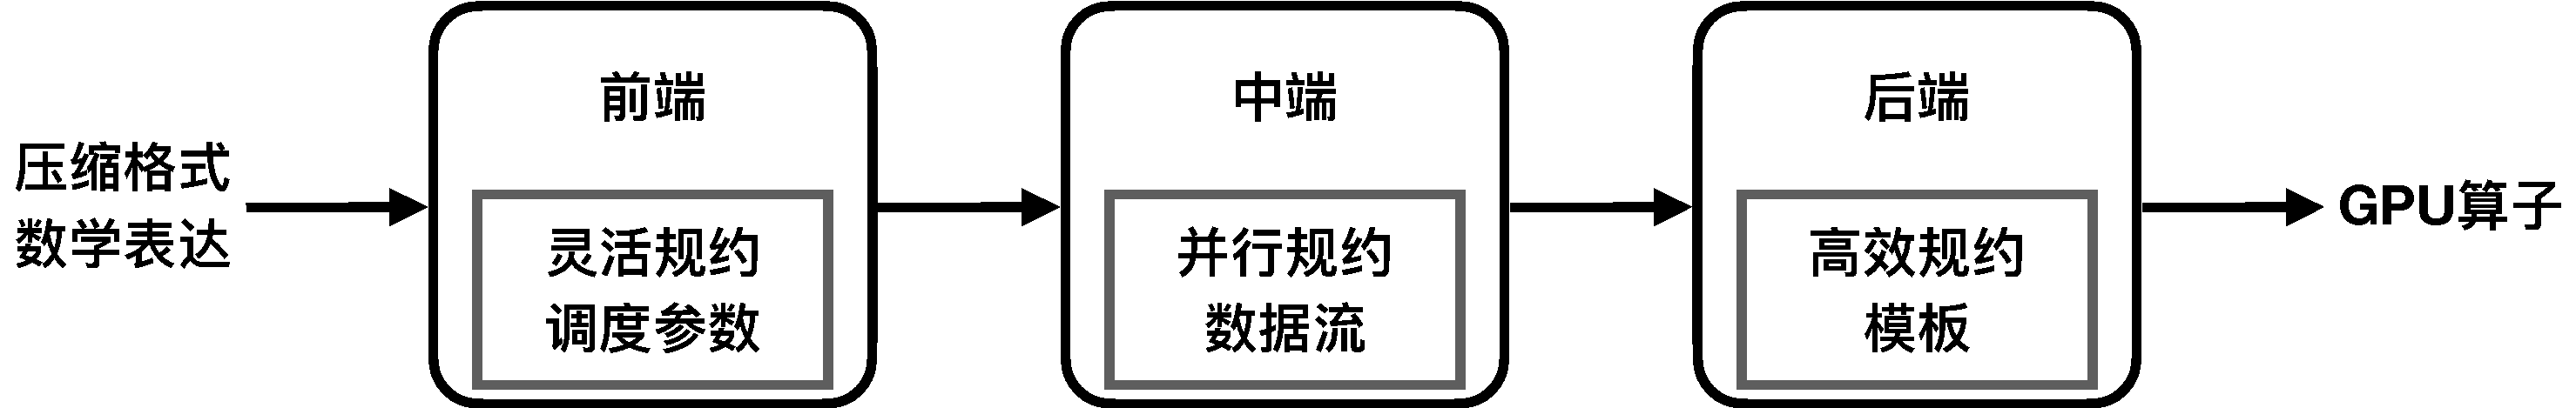
\includegraphics[width=0.99\textwidth]{overview.pdf}
  \caption{编译算法流程图}
  \caption*{圆角方框表示编译器功能模块层次,矩形方框表示本文添加的部分。}
  \label{fig:compiler-overview}
\end{figure}
\section{算法流程}
~\ref{sec:compiler-alg-intro}节提出灵活规约语义提升的两个内涵:线程组分块和同步语义分离,和同步语义灵活规约表达。实现这两个目标需要在前端、中端、后端三方面提出解决方案。具体而言,在前端引入新的并行计算单元抽象,并针对线程组的
分块语义设计新的调度指令。在中端,突破之前串行代码的语义分析逻辑,根据并行规约调整基本块和数据流。在后端,编写高效GPU线程组规约模板,并与中端的IR统一接口,使其执行前端输入的调度策略。以下以TACO编译器为例阐述这三部分编译算法,图
~\ref{fig:compiler-overview}总结了算法流程。
\subsection{前端}
在TACO中,前端提供了\textit{parallelize}接口表示并行计算,它定义为\textit{parallelize(IndexVar i, ParallelUnit pu, OutputRaceStrategy rs)}。这个变换使用并行计算单元$pu$在循环变量$i$上做并行执行。同时输出竞争策略$rs$
描述了在规约时发生的数据竞争。对GPU而言,$pu$可以是线程(GPUThread),线程组(GPUWarp)和线程块(GPUBlock),输出竞争策略$rs$可以是没有竞争(NoRaces),忽略竞争(IgnoreRaces)和原子操作(Atomics)。
为了实现分块和同步语义分离,添加新的并行计算单元(ParallelUnit):GPUGroup,用来描述并行度小于32的线程组并为其添加同步语义,同时取消并行计算单元GPUWarp的同步语义,仅保留分块语义。
具体而言,因为GPUWarp现在只作为分块中外部循环的线程编号,因此使用GPUWarp作为并行计算单元时取消了原子操作的输出竞争策略。同时,在使用GPUWarp时添加新的规约策略(ReductionStrategy)和线程组大小(GroupSize),并去掉输出竞争策略。
规约策略可以指定线程组的规约种类,比如~\ref{sec:flexible-reduciton}节中提到的分段规约和整体规约。GroupSize指定了规约并行度。
\subsection{中端和后端}
因为后端决定了中端的IR变换,同时二者通过IR连接,所以二者放在同一章节介绍。TACO提出一个稀疏张量算子编译器应该尽可能保证只有会产生非零输出的元素才会被计算。但是,在GPU灵活规约中,这一点并一定不成立。TACO的这个非零元素要求是在代码串行执行条件下的最优策略,因为在串行执行下,运算指令越少执行时间越短。
但是在SIMT架构下,规整但是计算量稍大的计算也可能快于计算量小但是不规整的计算。因此,在中端需要添加补零操作。与之搭配的技术成为零扩展。零扩展意味着向稀疏循环理论中添加一些超过边界的规约。这些规约之后会被后端的高效线程组规约模板执行,并且比for循环更快。
\begin{figure}[h]%
  \centering
  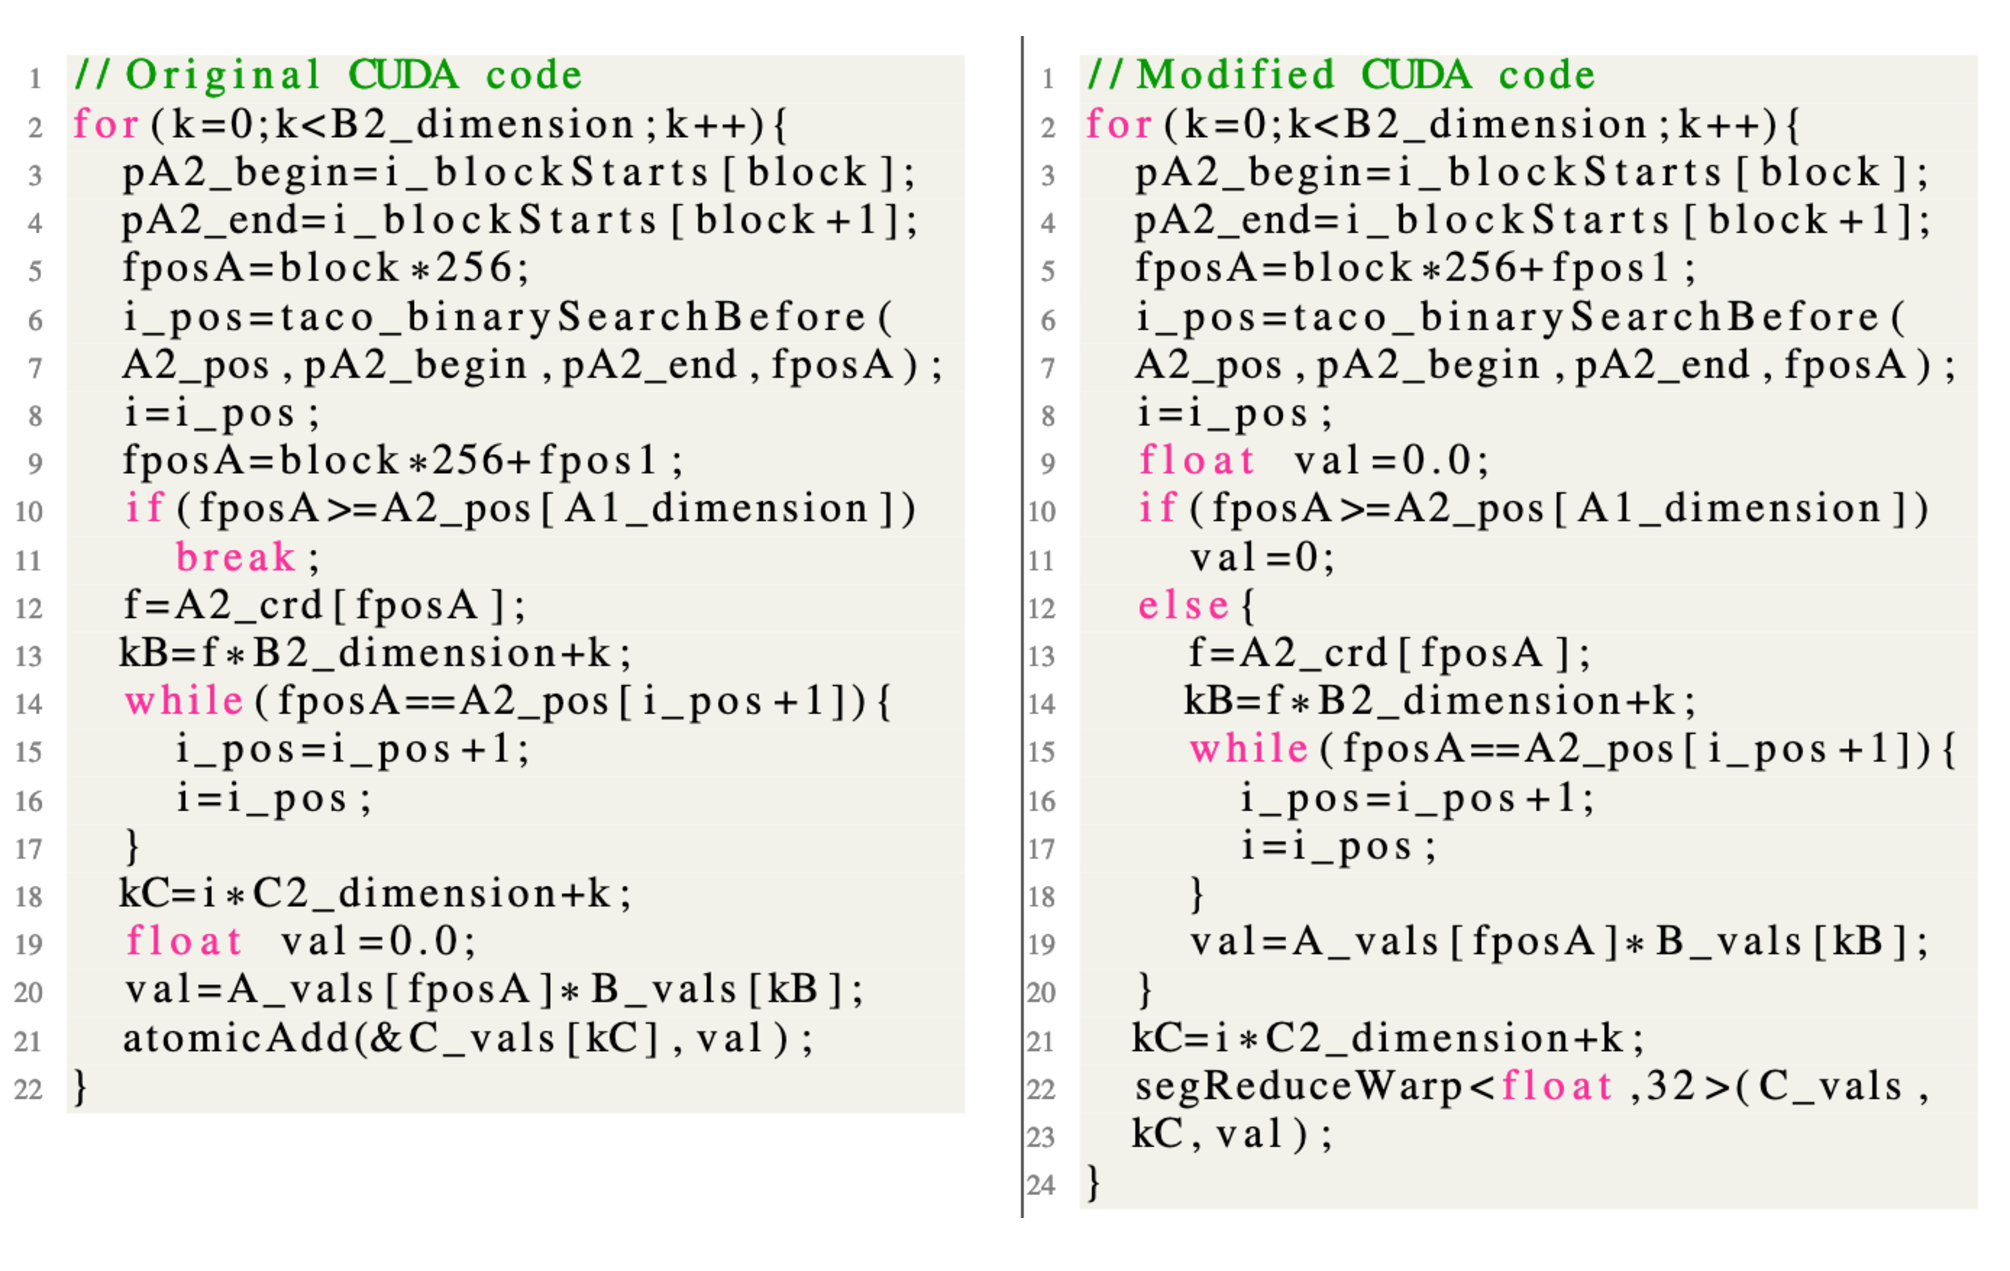
\includegraphics[width=0.99\textwidth]{code.pdf}
  \caption{生成CUDA代码示例}
  \caption*{左侧是修改前编译器生成的代码,右侧是利用灵活规约语义提升添加灵活规约扩展后编译器生成的代码.}\label{fig:code-example}
\end{figure}
图~\ref{fig:code-example}中对比了编译器修改前和修改后生成的代码。右侧代码使用GPUGroup作为并行计算单元,使用分段规约作为规约策略,使用32作为GroupSize,左侧代码使用GPUWarp作为计算单元,原子操作作为输出竞争策略,使用32作为分块粒度。除此之外,他们使用了相同的调度命令。二者有两处不同:标量转移空间,和宏指令。

标量转移空间:TACO假设标量转移空间的声明和赋值在同一个基本块中\cite{kjolstad:2019:workspaces}。这限制了TACO对于稀疏稠密张量计算的表达能力。例如,在$\{<1\,nnz , c\,col>,32\}$中,标量转移空间的赋值发生在属于else的基本块中,
但是标量转移空间的声明发生在和变量转移空间规约相同的上下文中。也就是声明发生在赋值的基本块外。如图~\ref{fig:controlflow}所示,为了实现零扩展,需要改变控制流。添加超过边界后的补零操作,同时将累计额和输出的功能集成到CUDA规约模板中。
\begin{figure}[h]%
  \centering
  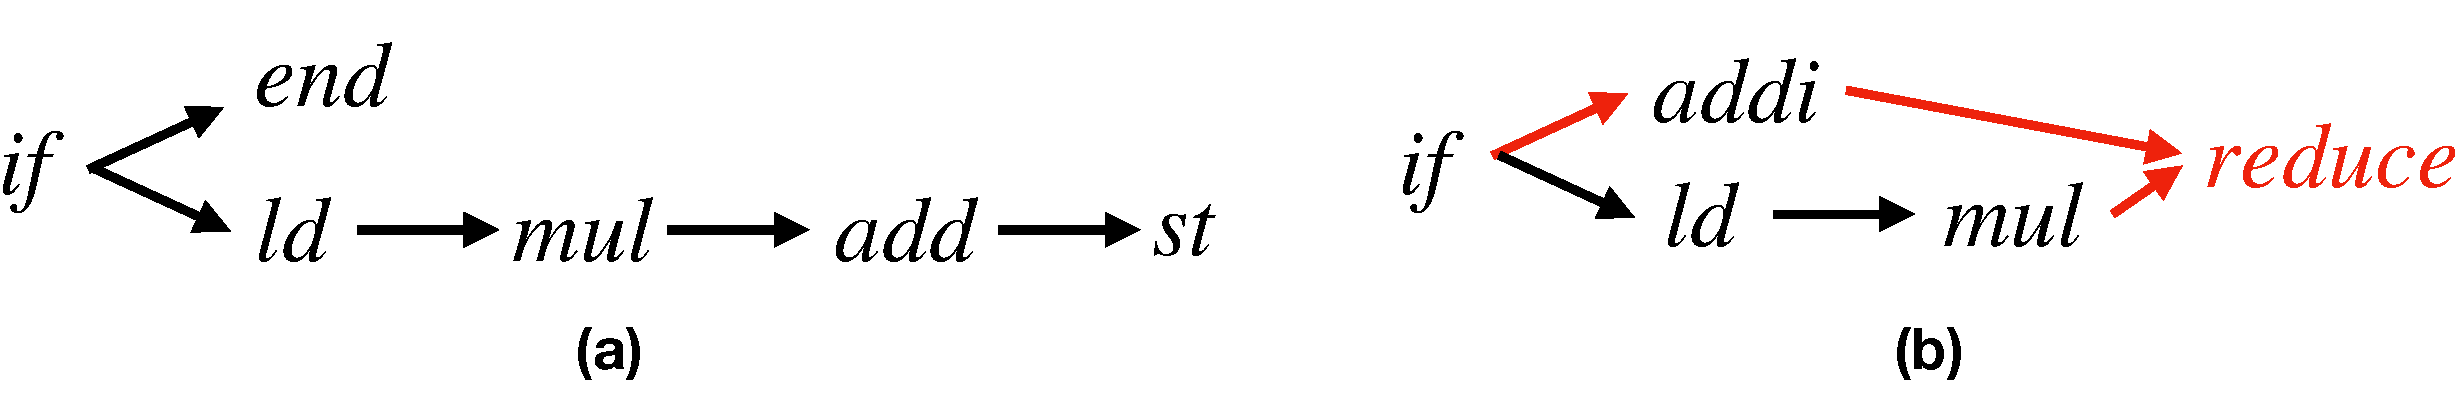
\includegraphics[width=0.99\textwidth]{controlflow.pdf}
  \caption{控制流变化示意图}
  \caption*{图(a)代表修改前的控制流,图(b)代表添加灵活规约语义提升后的控制流。其中if表示进行一个判断,if向上箭头表示条件满足后进入的基本块,向下箭头表示条件不满足进入的基本块。ld表示取数据,mul表示标量乘法,add表示标量加法,st表示存数据。addi表示含有一个常数的标量加法,这里用于实现零扩展。reduce表示一个线程组规约。因为规约中包含累加和存储操作,所以图(b)没有add和st。红色表示新增的操作和执行流。}
  \label{fig:controlflow}
\end{figure}
宏指令:我们希望设计模块化的代码生成系统,这样既利于简化上层IR变换,也利于CUDA指令更新。因为有一些特殊指令不能用于其他架构,所以不适合作为IR,而适合作为模版,其功能可以用上层IR描述,接口上暴露给上层一个简单的函数调用即可。
因此,我们设计了两个新的宏指令\textit{atomicAddGroup$<$T,G$>$(T* array, int idx, T value)}和\textit{segReducWarp$<$T,G$>$(T* array, int idx, T value)}。这两个模板函数的输入是输出向量的起始地址,输出的角标和需要被规约到输出的值。
他们将在G个线程中做规约,这里的G等于GroupSize。在具体实现上,他们会在头文件中声明,然后在最终的CUDA算子代码中作为宏指令被调用。事实上,部分灵活线程组技术来自于CUDA中的合作线程组(cooperaive group)特性。从CUDA11.0开始,CUDA开始支持易用的合作线程组
调用接口\footnote{\url{https://docs.nvidia.com/cuda/cuda-c-programming-guide/index.html\#cooperative-groups}},这使得在底层代码中控制小于32个线程粒度的同步,只需要实例化线程组对象然后调用相关方法。
\section{系统部署}
本节将以SpMM为例介绍灵活规约优化空间扩展在算子编译器中的部署和实现。我们将首先回顾TACO提出的两个SpMM算法,$\{<g\,nnz, c\,col>,1\}$和$\{<x\,row,c\,col >,1\}$。之后我们将使用$\{<\frac{1}{g}\,row, c\,col>,r\}$和$\{<1\,nnz , c\,col>,r\}$这两个例子展示具象角标表示(CIN)的变换过程。
SpMM的数学表达式$C(i,k) = A(i,j) * B(j,k)$。$A$的第一层是稠密格式,第二层是压缩格式。$B$和$C$都是稠密矩阵。$A,B,C$都是行优先存储的。在例子中我们会将$p,g,N,c$以字母形式填入CIN中来展示他们和CIN参数的运算关系。但是真实的CIN不会有没有确定的数值。
\subsection{已有优化空间}
当前TACO可以支持灵活规约扩展优化空间中的两类算法,$\{<g\,nnz, c\,col>,1\}$和$\{<x\,row,c\,col >,1\}$。因为其默认同步粒度是32,同时采用线程组整体规约,所以他们不需要同步语义,而只在分块语义层面进行性能调优。两种算法各自的CIN如图~\ref{fig:CIN-1}和图~\ref{fig:CIN-2}所示
它们强制要求同步粒度是1,因此限制了规约的优化空间。针对$\{<g\,nnz, c\,col>,1\}$,我们采用~\ref{sec:spcomp}节介绍的角标表示重写类生层如图~\ref{fig:CIN-1}所示的CIN。在~\cite{senanayake:2020:scheduling}中,采用$N=128,g=16,c=4,p=512$进行性能实验。
针对$\{<x\,row,c\,col >,1\}$,我们直接使用TACO命令行工具即可生成,在~\cite{senanayake:2020:scheduling}中,采用$N=128,g=1,c=4,p=512$进行性能实验。这两种算法都只用到了GPUWarp的分块语义。
\begin{figure}[h]%
  \centering
  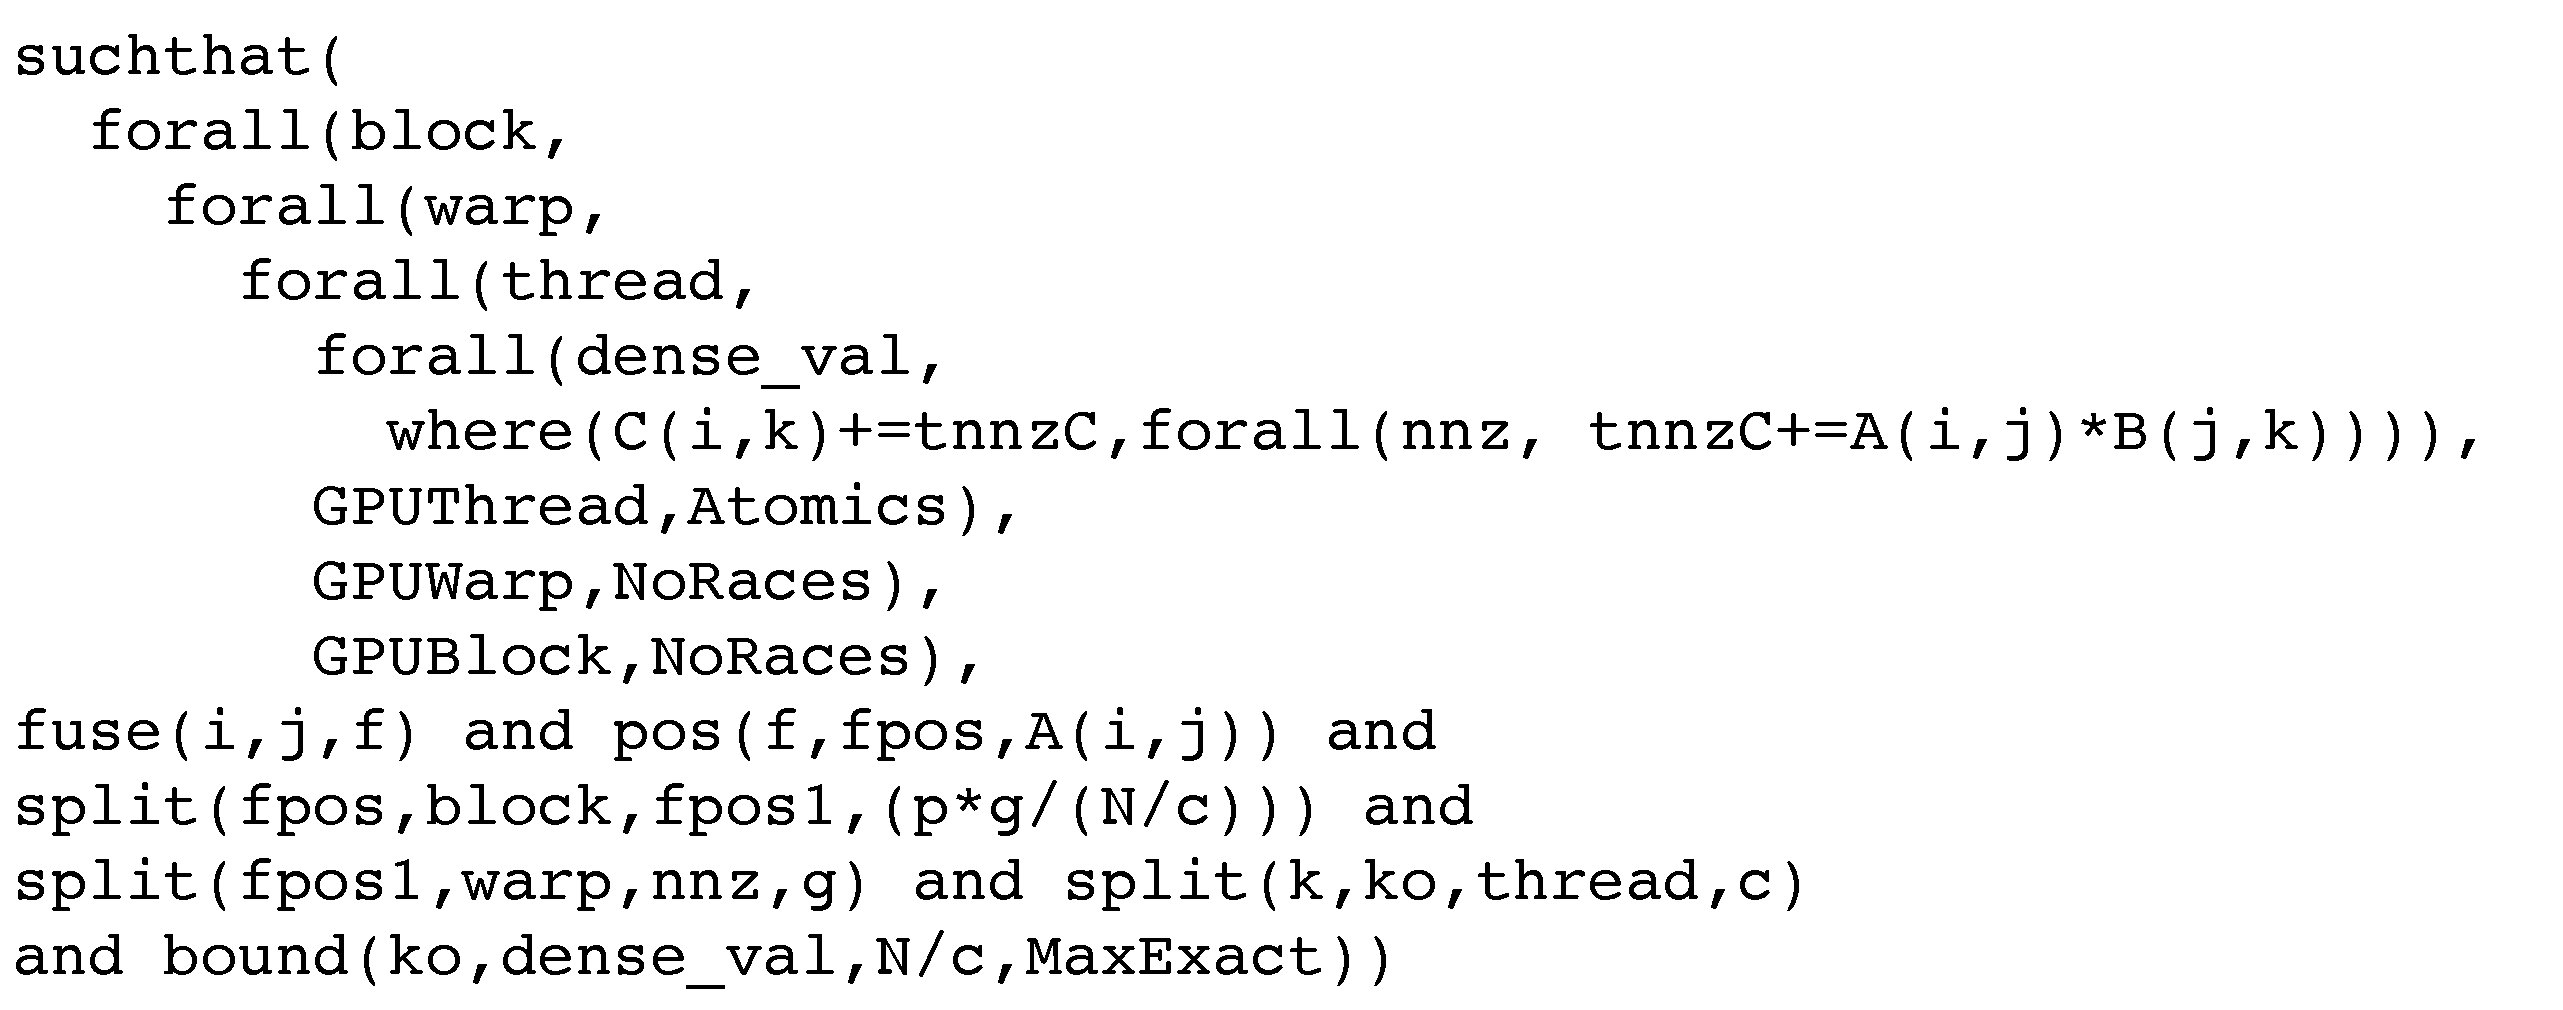
\includegraphics[width=0.99\textwidth]{CIN-1.pdf}
  \caption{$\{<g\,nnz, c\,col>,1\}$的CIN}\label{fig:CIN-1}
\end{figure}
\begin{figure}[h]%
  \centering
  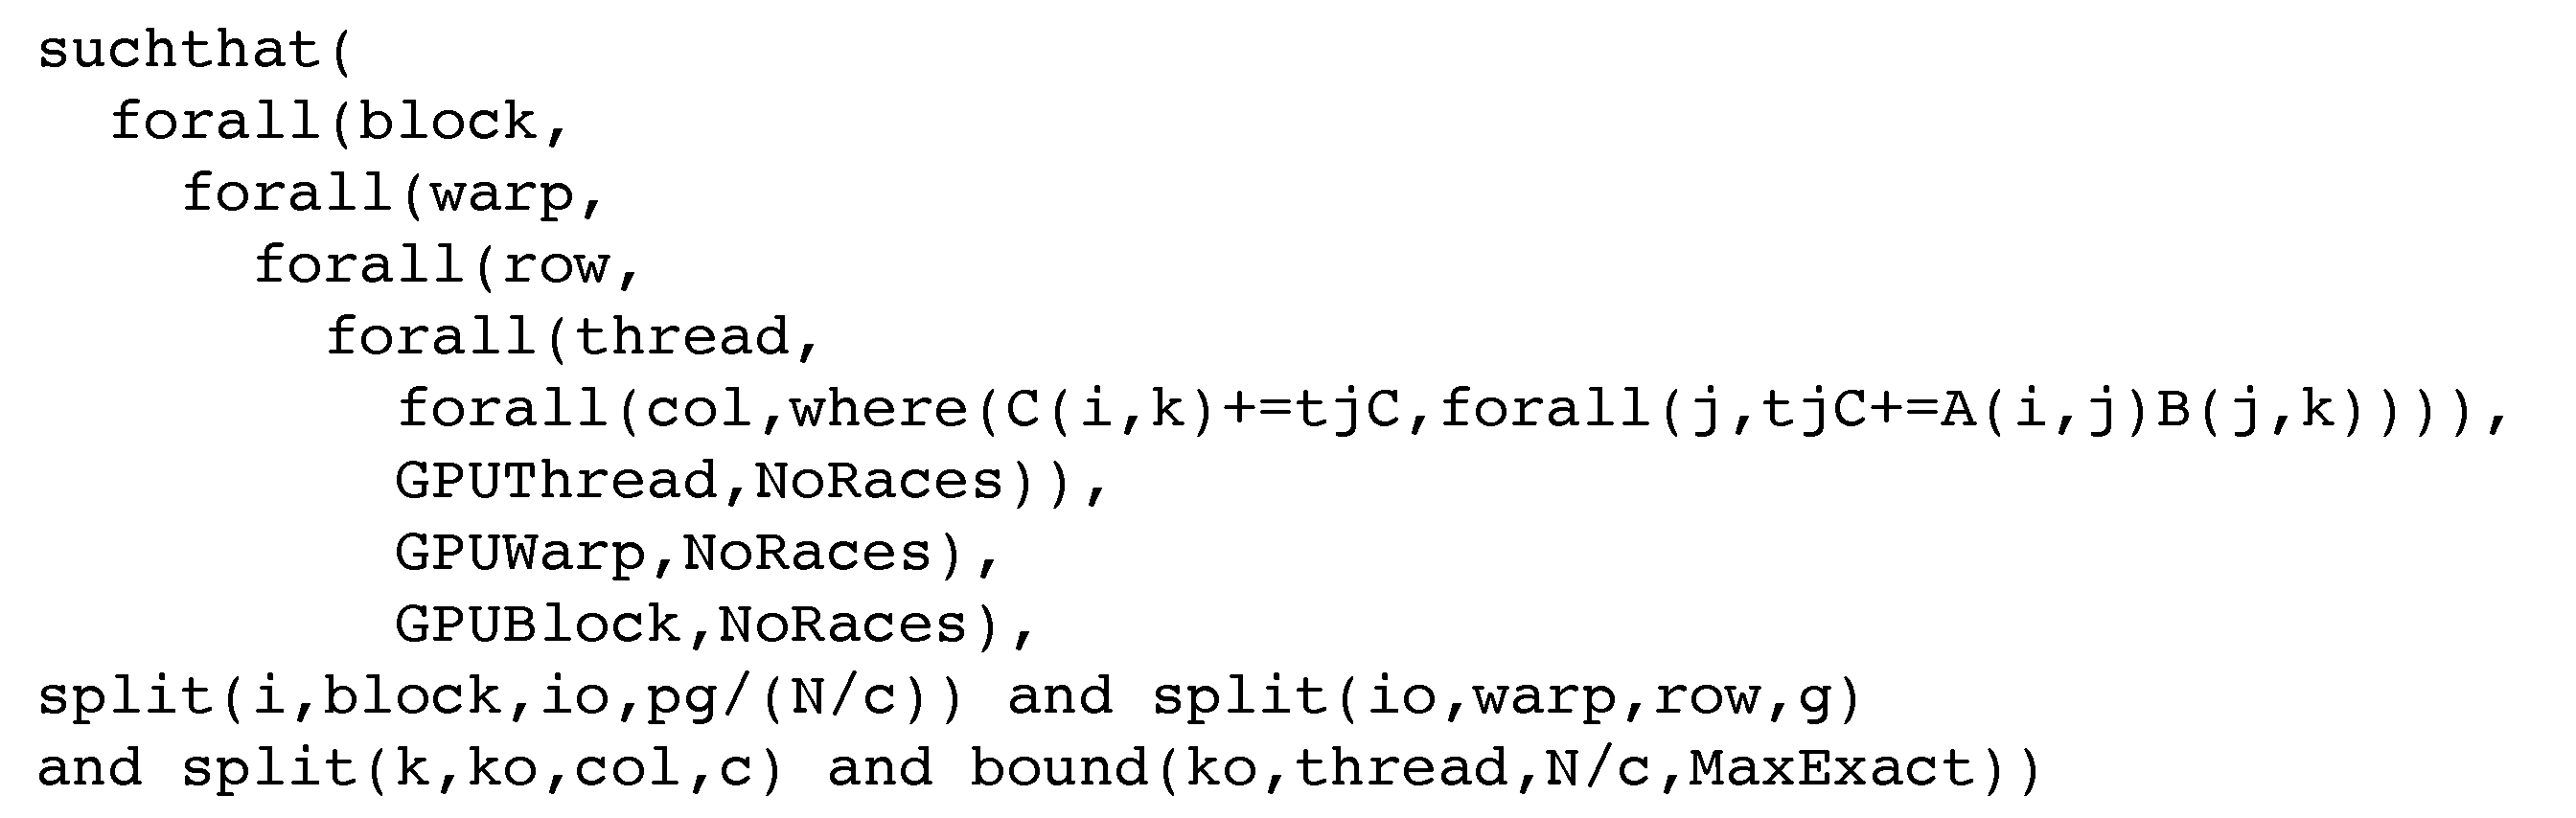
\includegraphics[width=0.99\textwidth]{CIN-2.pdf}
  \caption{$\{<x\,row,c\,col >,1\}$的CIN}\label{fig:CIN-2}
\end{figure}
\subsection{扩展优化空间}\label{sec:comp-space}
将灵活规约扩展优化空间中的$\{<\frac{1}{g}\,row, c\,col>,r\}$和$\{<1\,nnz , c\,col>,r\}$引入稀疏算子编译器可以提升工作负载均衡。如图~\ref{fig:CIN-3}和图~\ref{fig:CIN-4}所示,这两种算法提供了变换线程组大小和规约策略的功能。用户可以针对非零元和行数的性能调优。
\begin{figure}[h]%
  \centering
  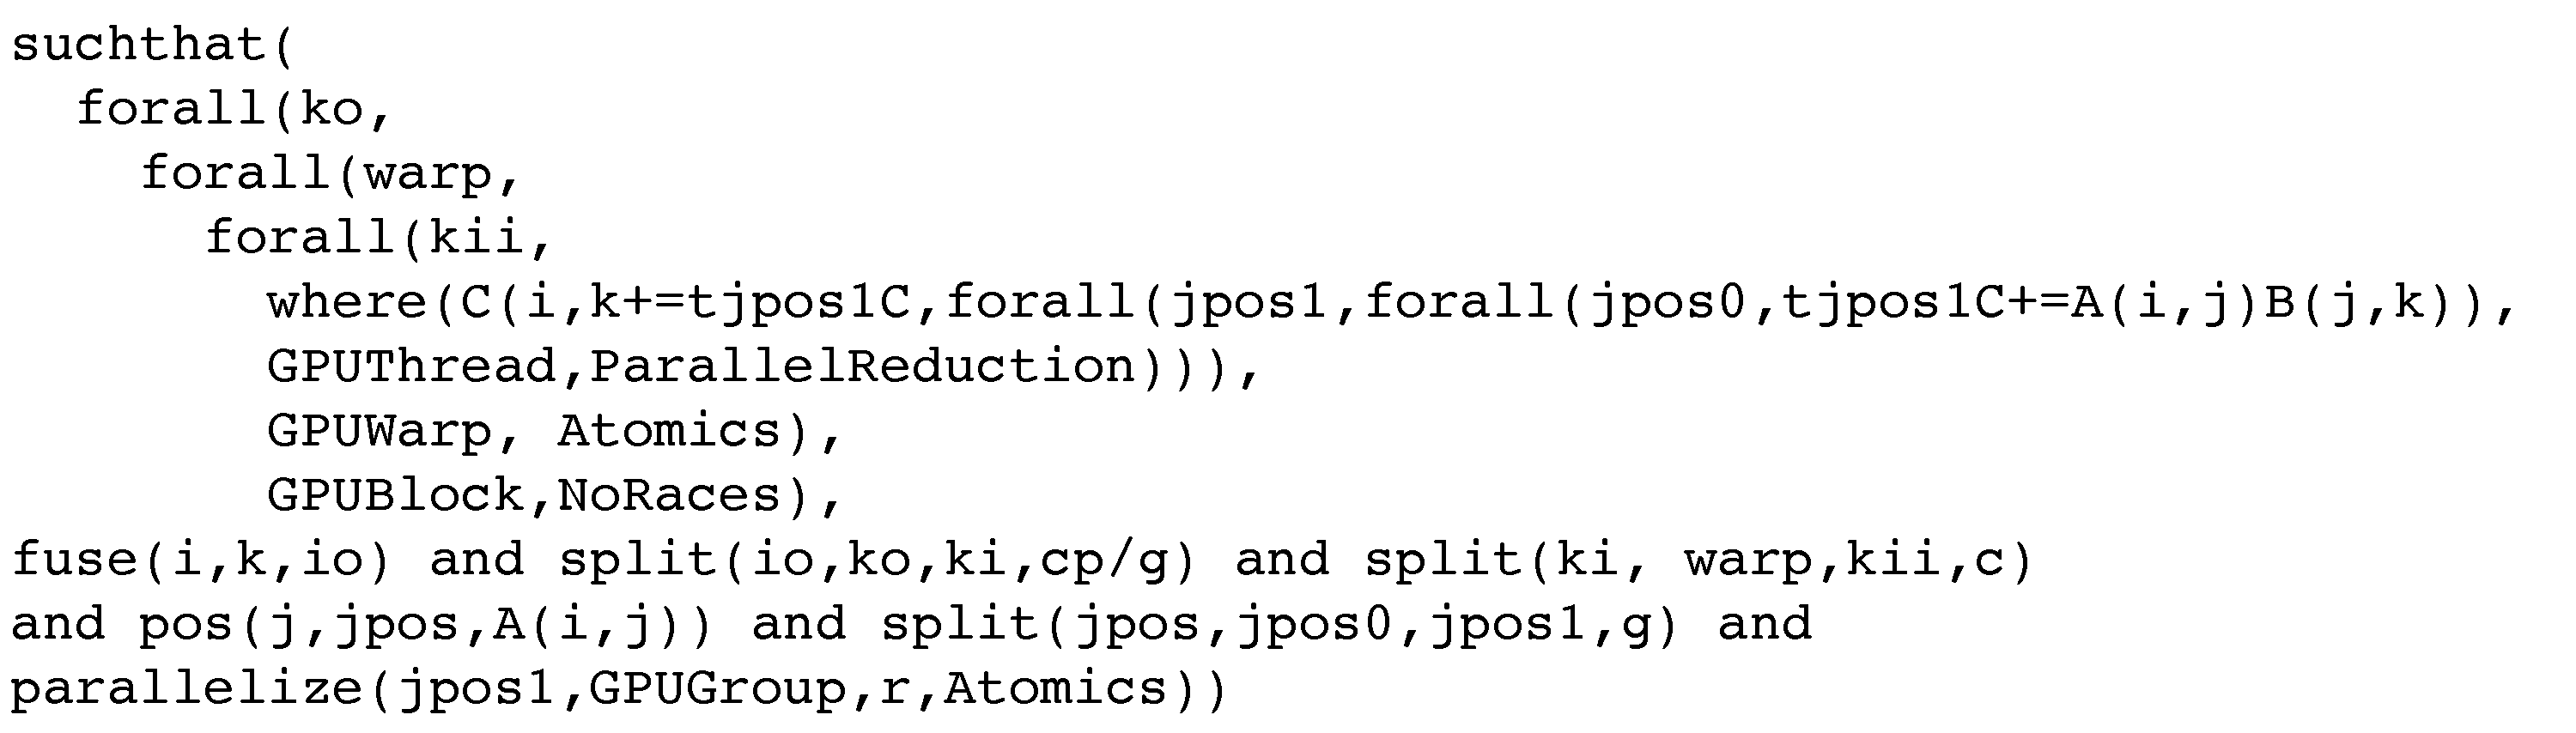
\includegraphics[width=0.99\textwidth]{CIN-3.pdf}
  \caption{$\{<\frac{1}{g}\,row, c\,col>,r\}$的CIN}\label{fig:CIN-3}
\end{figure}
\begin{figure}[h]%
  \centering
  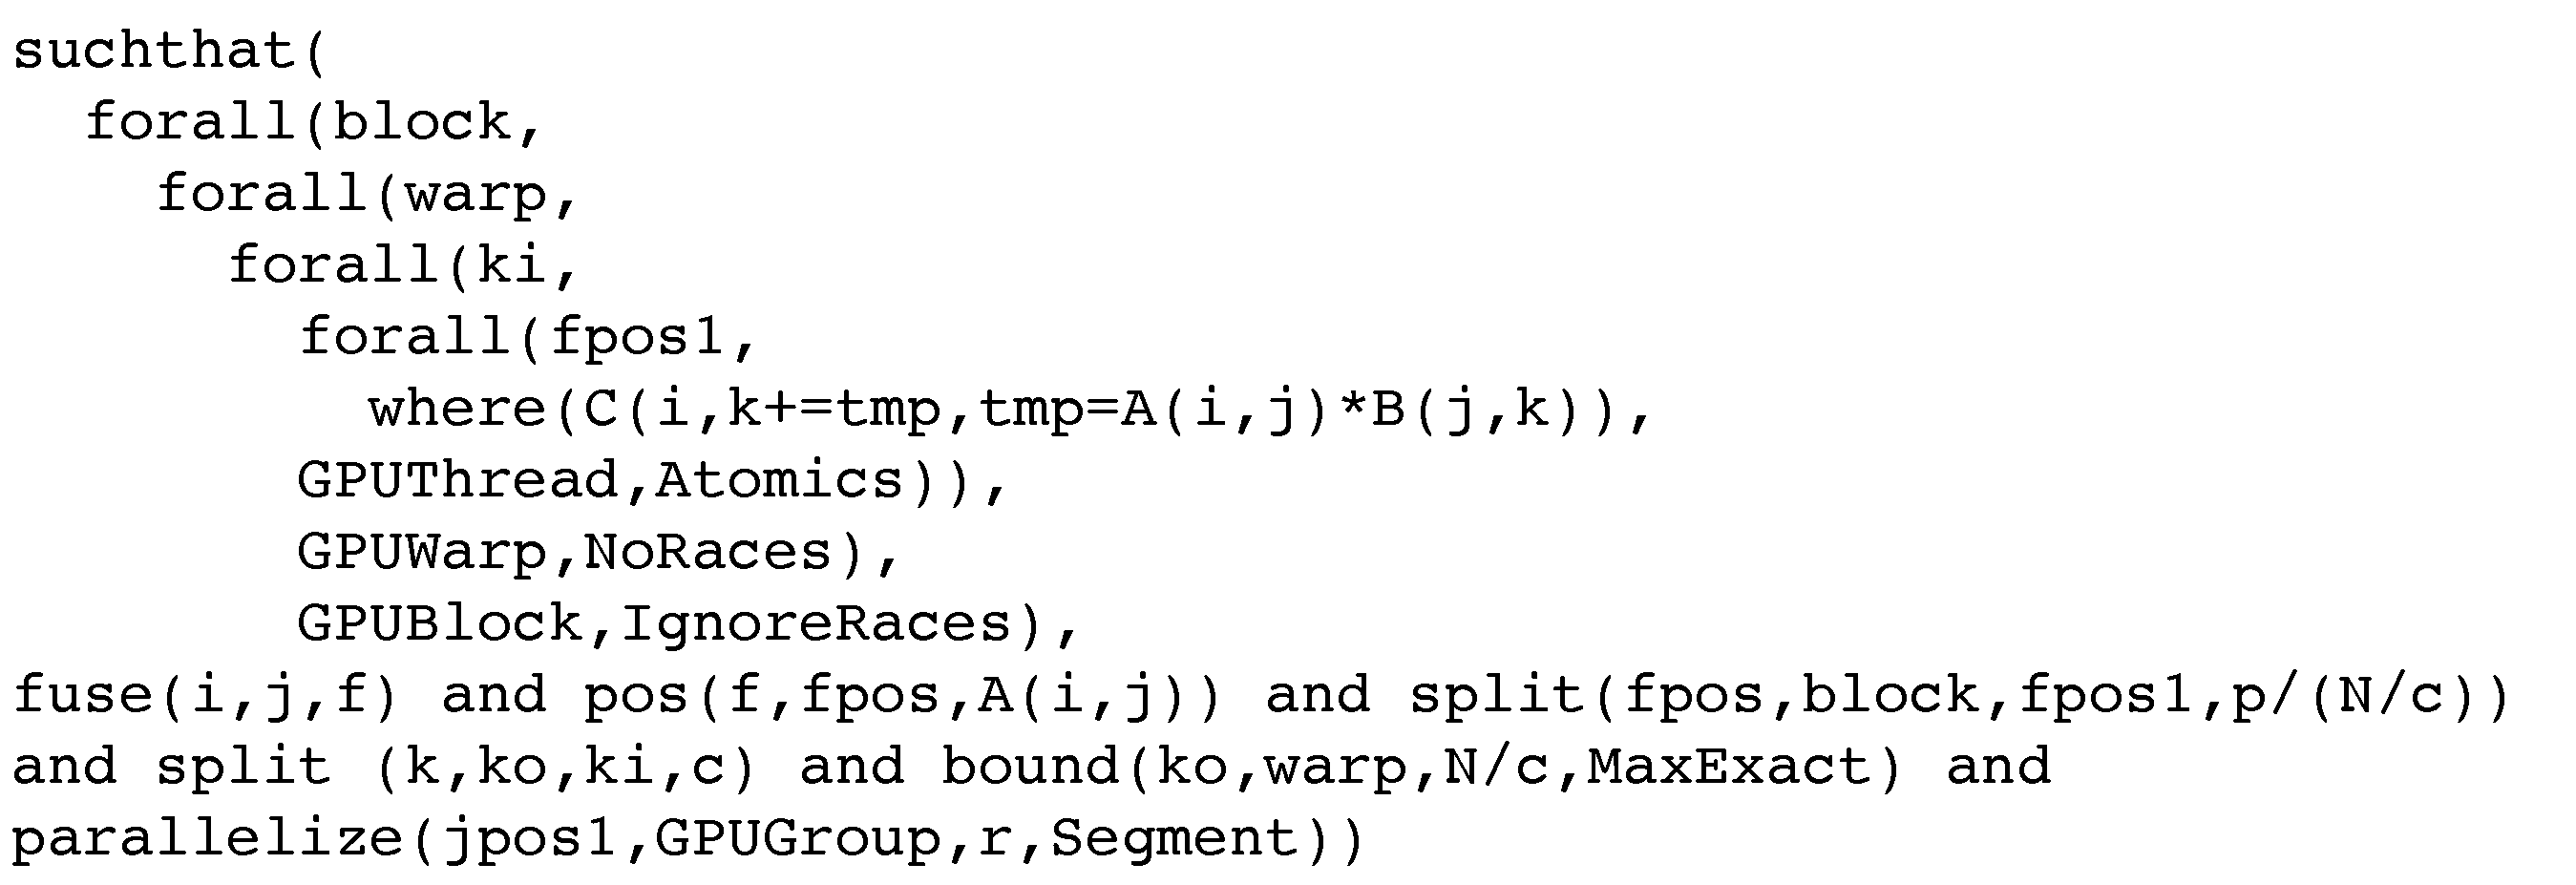
\includegraphics[width=0.99\textwidth]{CIN-4.pdf}
  \caption{$\{<1\,nnz , c\,col>,r\}$的CIN}\label{fig:CIN-4}
\end{figure}
实际上TACO可以支持$g=32, r=32$的$\{<\frac{1}{g}\,row, c\,col>,r\}$算法,但是TACO不能支持其他参数的该种算法。GPUGroup被完成规约的循环变量所限制。原本生成的宏指令\textit{atomicAddWarp$<$Type$>$}被替换成\textit{atomicAddGroup$<$Type, G$>$}来处理更细粒度的线程同步。
图~\ref{fig:CIN-4}展示的$\{<1\,nnz , c\,col>,r\}$算法在原本的TACO中没有被支持。我们将原本发射的\textit{atomicAdd}替换成\textit{segReduceGroup$<$Type,G$>$},分段规约就在新的宏指令中完成。标量转移空间的中端变换也被转换成可以执行分段规约的数据流。

\section{实验结果}
实验环境和~\ref{sec:exp-env}节中相同。本节实验用于证明灵活规约语义提升技术可以提高稀疏算子编译器的优化空间表达能力,并提高编译器生成算子的质量。在实验中未明确指出时稠密矩阵列数N默认为4。
\subsection{灵活规约粒度和静态规约粒度对比}
我们使用$\{<\frac{1}{g}\,row, c\,col>,r\}$来展示引入灵活规约粒度后带来的算子性能提升。如~\ref{sec:comp-space}节提到的,当前TACO只支持$g=32, r=32$。因此我们控制$g$为与TACO相同的32,并改变$r$。在表~\ref{tab:comp-flexgra}中展示了$r=8$和$r=4$可以给原有算子带来超过2倍的性能提升。
其中A相对于B的后验性能提升表示,当A比B的性能更好时,记录加速比;当A的性能不如B时,加速比记为1。这种统计方式展示了添加自动性能调优器后灵活规约带来的性能提升上限。
\begin{table}
  \centering
  \caption{灵活规约粒度对比静态规约粒度性能提升}
  \begin{tabular}{llllll}
  \toprule
  硬件平台 &  $r=8$  & $r=8$后验 & $r=4$  & $r=4$后验\\
  \midrule
  RTX 2080    & 2.451   & 2.478 & 2.456 & 2.483 \\
  RTX 3090    & 2.236   & 2.284  & 2.259 & 2.307 \\
  Tesla V100    & 2.086  & 2.143  & 2.094 & 2.150 \\
  \bottomrule
  \end{tabular}
  \label{tab:comp-flexgra}
\end{table}
\subsection{灵活规约策略和单一规约策略对比}
我们使用$\{<1\,nnz , c\,col>,r\}$来展示灵活规约策略带来的性能提升。本节以分段规约和整体规约为例,因为他们有不同的数据类别(非零元与行),因此我们控制$c$和$r$相同,并将$\{<1\,nnz , c\,col>,r\}$与改变$g$得到的最优的$\{<\frac{1}{g}\,row, c\,col>,r\}$的性能。
这一实验只在RTX 3090上完成,此处记录的是后验加速比。在表~\ref{tab:comp-flexstr}中展示了分段规约可以比之前TACO中采用的整体规约加速1.3倍。受限于GPU提供的最大线程组大小为32,所以$r$只能是$1,2,4,8,16,32$。因此,在实际使用中用户可以尝试使用这些数字对$r$进行性能调优。
\begin{table}
  \centering
  \caption{灵活规约策略对比单一规约策略性能提升}
  \begin{tabular}{llllll}
  \toprule
  c &  $r=4$  & $r=8$ & $r=16$  & $r=32$\\
  \midrule
  1   & 1.008   & 1.025  & 1.085 & 1.272 \\
  2    & 1.019   & 1.045  & 1.102 & 1.291 \\
  4   & 1.063   & 1.095  & 1.205 & 1.381 \\
  \bottomrule
  \end{tabular}
  \label{tab:comp-flexstr}
\end{table}
\subsection{灵活规约与优化前编译器对比}
在这一实验中,我们对比TACO的原始SpMM算法$\{<g\,nnz, c\,col>,1\}$和$\{<x\,row,c\,col >,1\}$,以及灵活规约语义提升新增的$\{<\frac{1}{g}\,row, c\,col>,r\}$和$\{<1\,nnz , c\,col>,r\}$。
各种算法中的$g,c,x,$和$r$参数被赋予合理的值并进行性能调优。我们记录了每种算法在每个数据集上的后验最佳性能。从表~\ref{tab:comp-all}中我们可以得出灵活规约可以生成1.1倍到1.2倍更快的算子。同时,我们也
测试了不同稠密矩阵列数下的实际性能提升(即非后验性能)。如图~\ref{fig:comp-tables}所示,可以发现稠密矩阵列数越小,灵活规约的优势越大。
\begin{table}
  \centering
  \caption{灵活规约与优化前编译器生成算子后验性能对比}
  \begin{tabular}{lllll}
  \toprule
  & RTX 3090  & RTX 2080 & Tesla V100 \\
  \midrule
  加速比   & 1.191   & 1.098  & 1.223\\
  \bottomrule
  \end{tabular}
  \label{tab:comp-all}
\end{table}
\begin{figure}[h]%
  \centering
  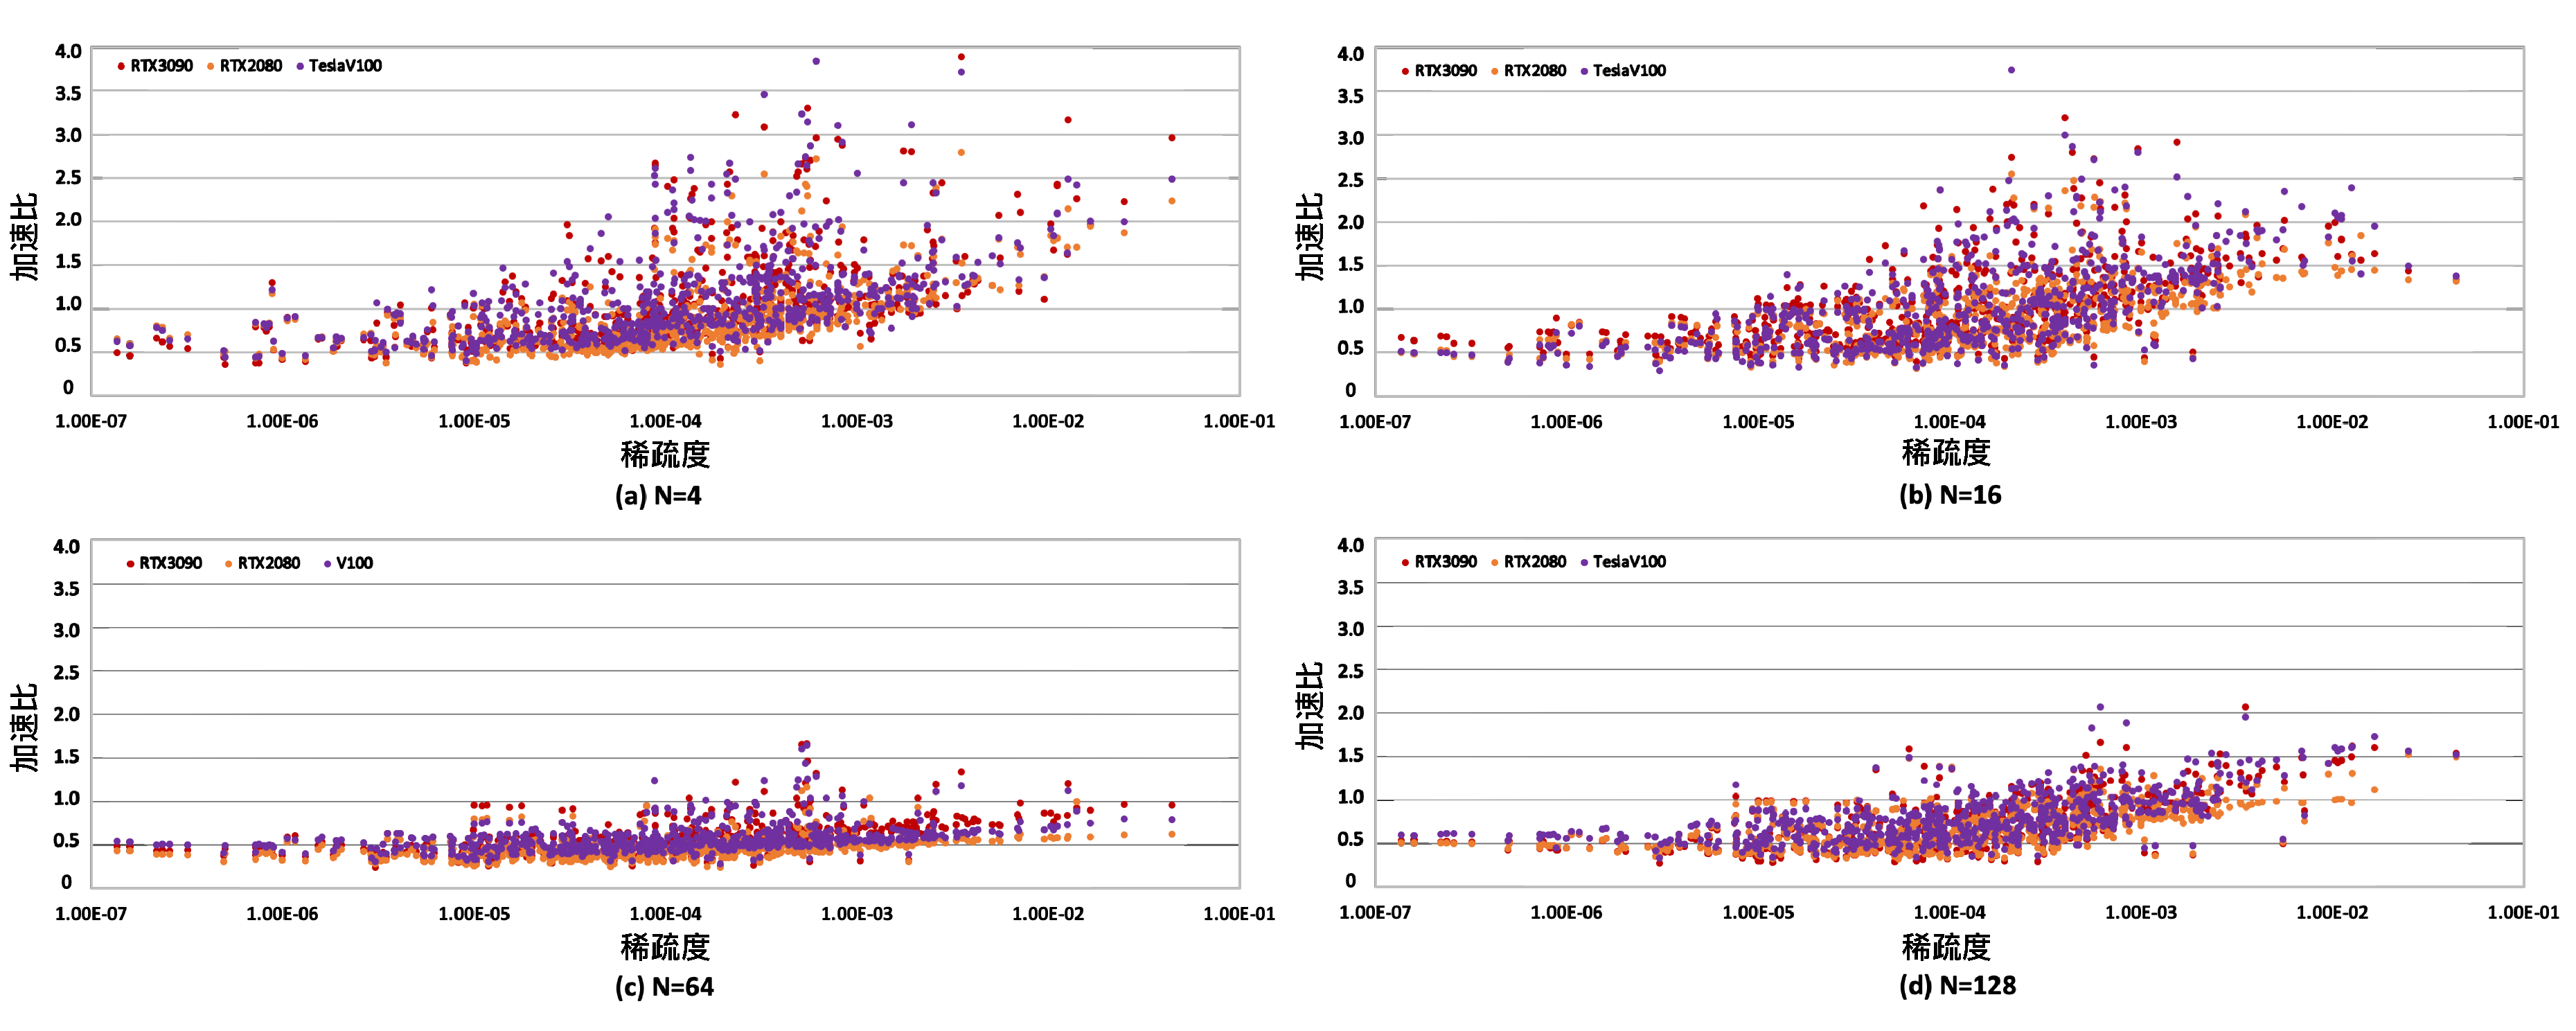
\includegraphics[width=0.99\textwidth]{new_tables-cn.pdf}
  \caption{不同稠密矩阵列数下灵活规约与优化前编译器生成算子性能对比}
  \caption*{稀疏度定义为稀疏矩阵中非零元个数除以行数和列数的乘积。}
  \label{fig:comp-tables}
\end{figure}
\subsection{灵活规约优化泛化性}
\begin{longtable}{ccccc}
  \caption{MTTKRP测试张量信息}
  \label{tab:tensor-info} \\
  \toprule
  张量名称& 第一维  & 第二维 & 第三维 & 稀疏度 \\
  \midrule
  \endfirsthead
  \caption*{续表~\thetable\quad MTTKRP测试张量信息} \\
  \toprule
  张量名称& 第一维  & 第二维 & 第三维 & 稀疏度 \\
  \midrule
  \endhead
  \bottomrule
  \endfoot
  1998DARPA   & 22K  & 22K & 23K  & 2.37E-09\\
  amazon-reviews   & 4.8M  & 1.7M & 1.8M  & 1.13E-10\\
  delicious-3d   & 0.53M  & 17M & 2.5M  & 6.14E-12\\
  flickr-3d   & 0.32M  & 28M & 1.6M  & 7.8E-12\\
  freebase\_music   & 23M  & 23M & 0.17K  & 1.10E-09\\
  freebase\_sampled   & 39M  & 39M & 0.53K  & 1.73E-10\\
  nell-2   & 12K  & 9.2K & 29K  & 9.05E-13\\
  nell-1   & 0.32M  & 28M & 1.6M  & 9.05E-13\\
\end{longtable}

\begin{figure}[H]%
  \centering
  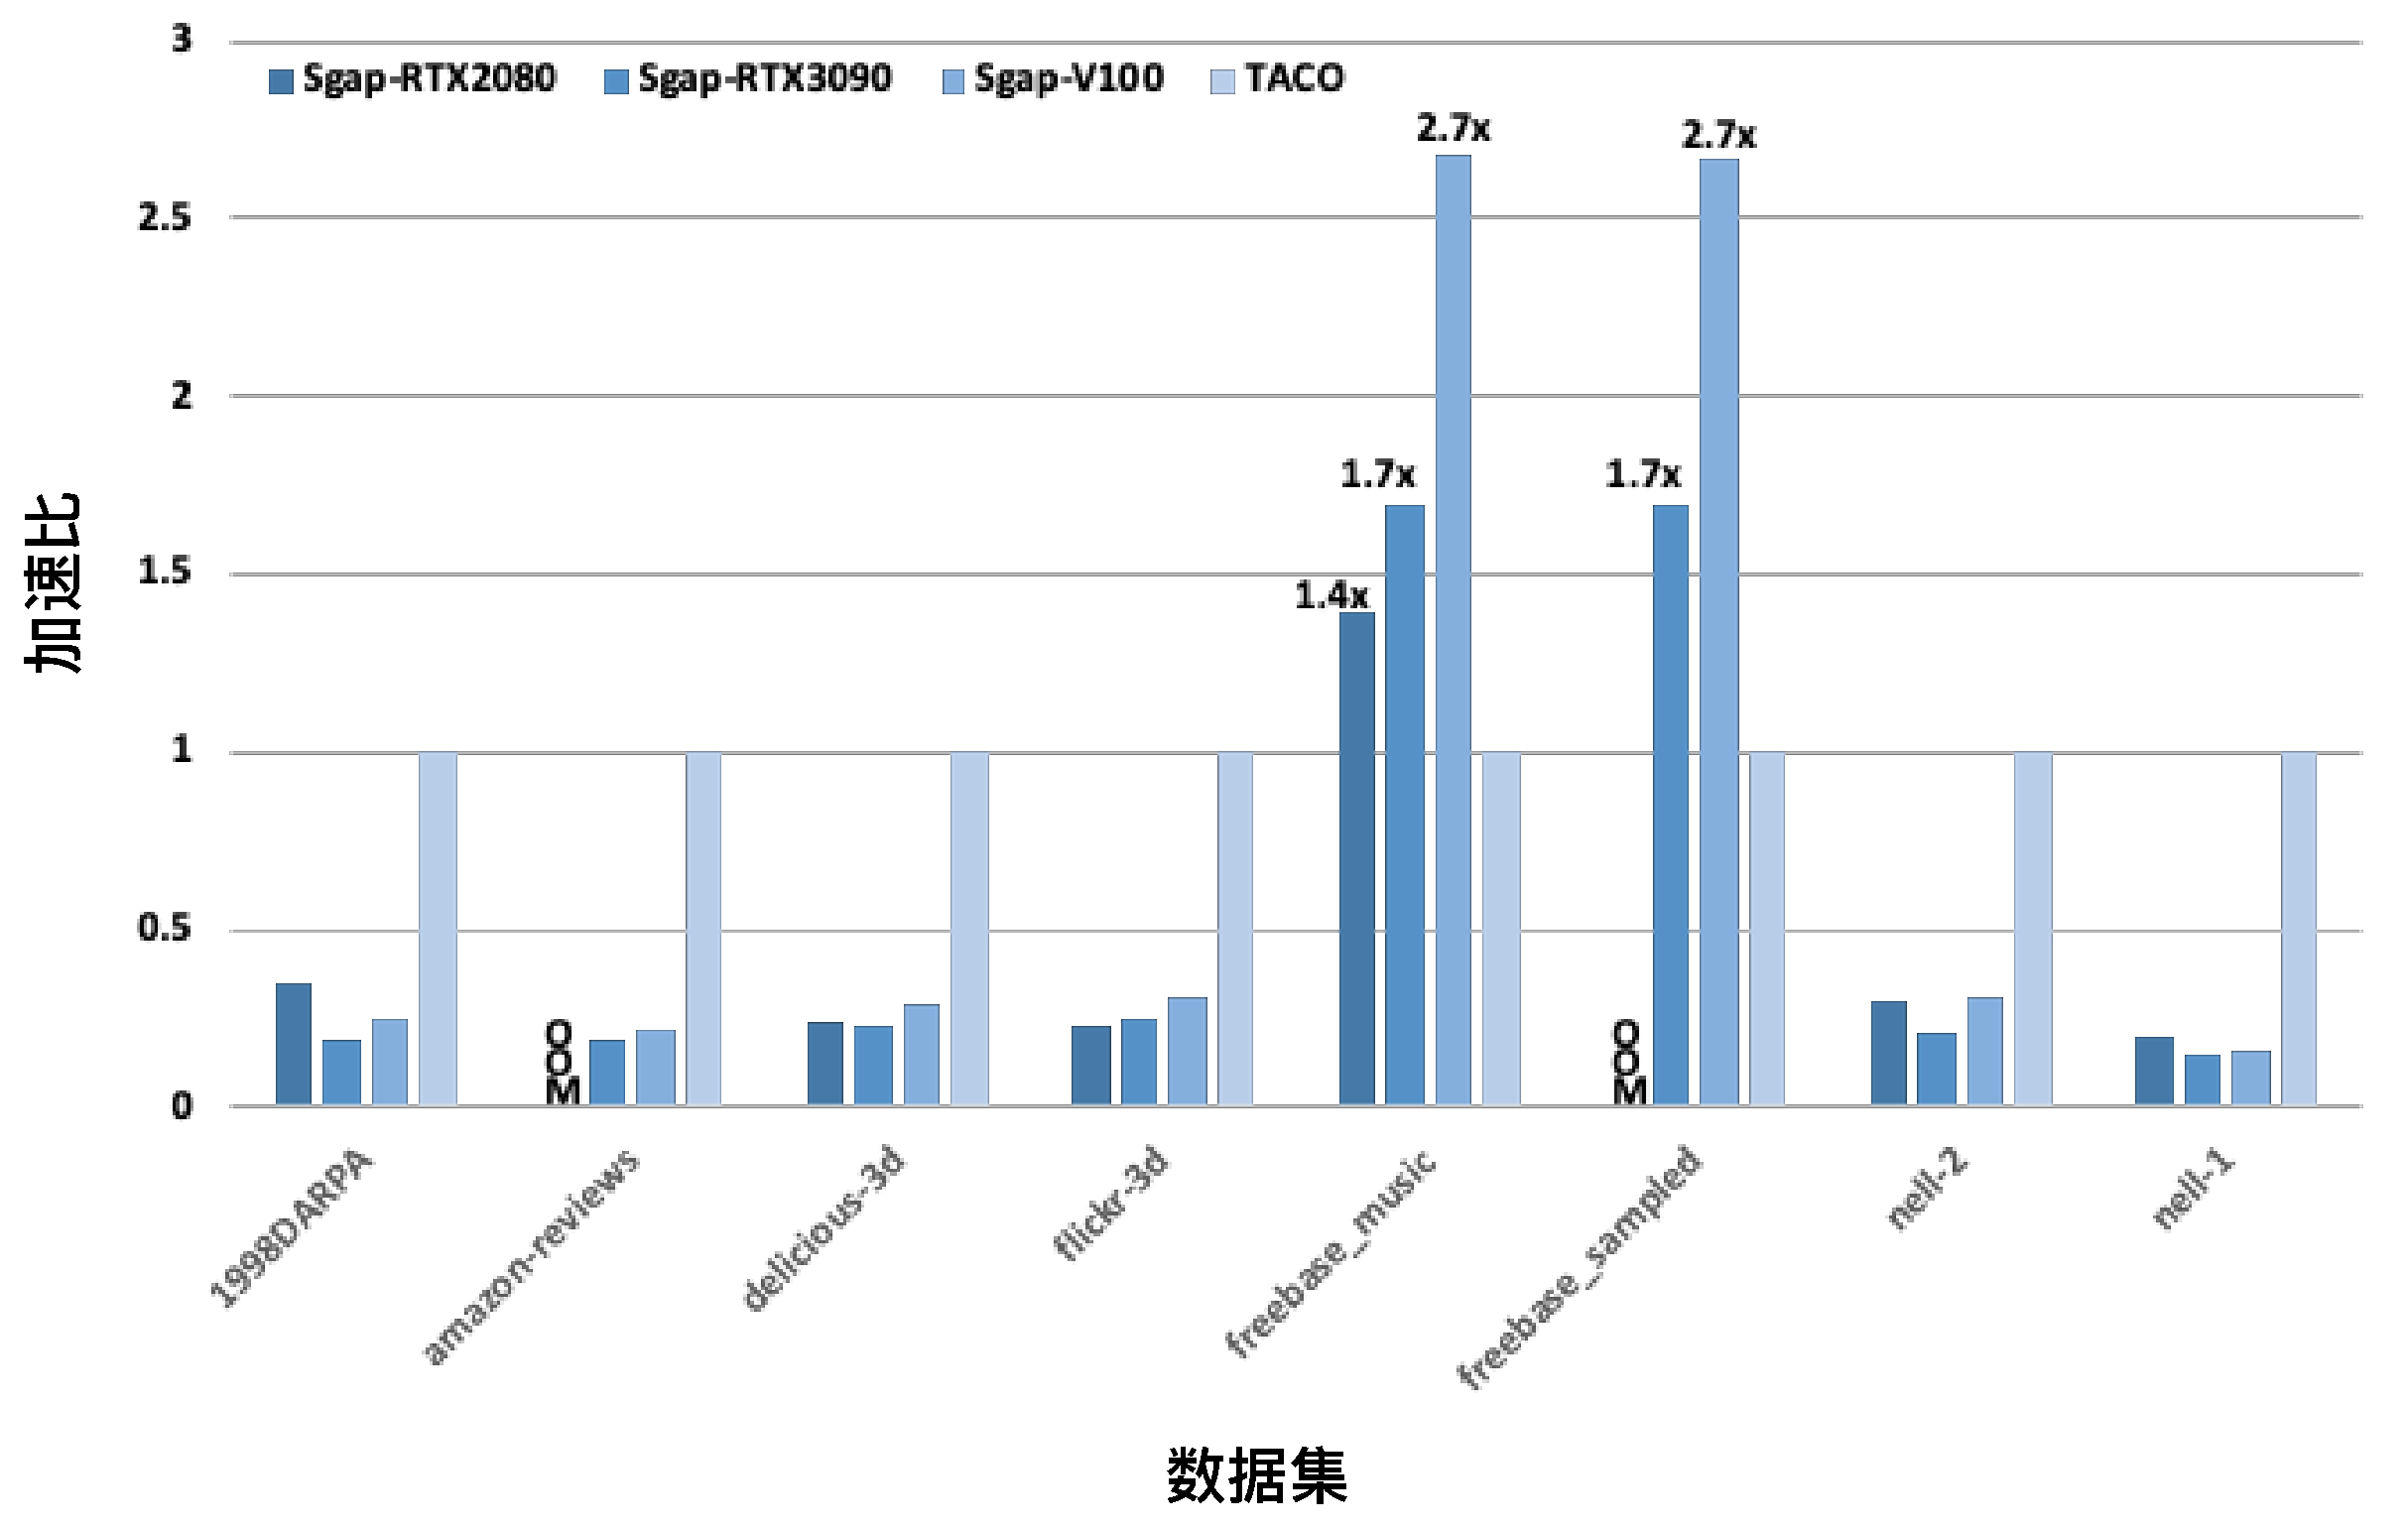
\includegraphics[width=0.99\textwidth]{mttkrp.pdf}
  \caption{MTTKRP在不同数据集下灵活规约和编译器原有算法生成算子性能对比}
  \caption*{图中OOM(Out-Of-Memory)表示算子运行过程中显存溢出。}
  \label{fig:comp-mttkrp}
\end{figure}

优化泛化性是指除了自身的优化对象,一种优化技术可以加速其他算子。在~\ref{sec:reduction-core}节中分析了优化规约就可以加速稀疏稠密混合代数。本节以MTTKRP为例,通过实验表明灵活规约的优化泛化性。采用和~\cite{senanayake:2020:scheduling}中相同的
调度指令,只是规约部分改成灵活规约。表~\ref{tab:tensor-info}展示了测试所用三维稀疏张量的基本信息。高维稀疏张量数据较为稀缺,这里选取的8个三维稀疏张量是常用的开源稀疏张量数据。图~\ref{fig:comp-mttkrp}展示了MTTKRP在freebase\_music和freebase\_sampled这两个数据集上可以获得最高2.7倍的性能提升。